% created on 27/11/2020
% @author : ebazan

\chapter{Perceptual Object Segmentation Model} \label{ch:perceptual_object_boundaries_detection}

\section*{Résumé}
\noindent Dans ce chapitre, nous utilisons les concepts développés tout au long de la thèse pour générer un modèle de segmentation d'image non supervisée. Le modèle est basé sur la décomposition multispectrale de l'image transformée en un espace colorimétrique luminance-chrominance. Nous représentons l'image sous forme de graphique et avec la métrique EMD nous générons un gradient perceptif à partir duquel nous obtenons les contours perceptives de l'image. Les résultats des contours et de la segmentation générés par la méthodologie proposée sont comparés aux différentes travaux de l'état de l'art.
\section*{Abstract}
\noindent In this chapter we make use of the concepts developed throughout the thesis to generate a model for unsupervised image segmentation. The model is based on the multispectral decomposition of the image transformed into a luminacy-chrominance color space. We represent the image as a graph and with the EMD metric we generate a perceptual gradient from which we obtain the perceptual boundaries of the image. The results of boundaries and segmentation generated by the proposed methodology are compared with the different works of the state of the art.

\section{Introduction}
In Chapters \ref{ch:spectral_image_decomposition} and \ref{ch:complex_spectral_image_decomposition} we have introduced the theoretical aspects of gabor filters and their use in a complex color space. Using the family of filters as a measurement tool, we create a feature space that exploits the color and texture information of the images and the relationship between them. This feature space can be seen as the complex spectral decomposition of an image.

In this chapter we propose a workflow to use it in the image segmentation task. We have seen that it is possible to obtain unsupervised segmentation using some clustering methods on the proposed feature space (see Chapter \ref{ch:complex_spectral_image_decomposition}). However, clustering methods have the limitation of needing some kind of a priori information, for example the number of clusters or objects in the image. The objective of the proposed framework is to obtain a coherent segmentation of the image using the fewest possible parameters.

The present framework obtains the segmentation of an image from the perceptual gradient of the objects. The overall idea of our framework can be seen in the diagram of figure \ref{fig:pipeline_gabor_image_segmentation}. First, we represent the image as a graph (which can be pixel-based or region-based). Next, we calculate the graph's edge's weight using the concept of optimal transport through the EMD (see section \ref{subsec:EMD}), which is a measure that reflects the true distance between two distributions. Finally, the representation of the image as an edge-weighted graph allows to straightforward apply various graph-based segmentation techniques or, to recover the perceptual boundaries of the image in the form of a gradient image, on which we can apply some boundary-based segmentation techniques.


\begin{figure}[!ht]
	\centering
	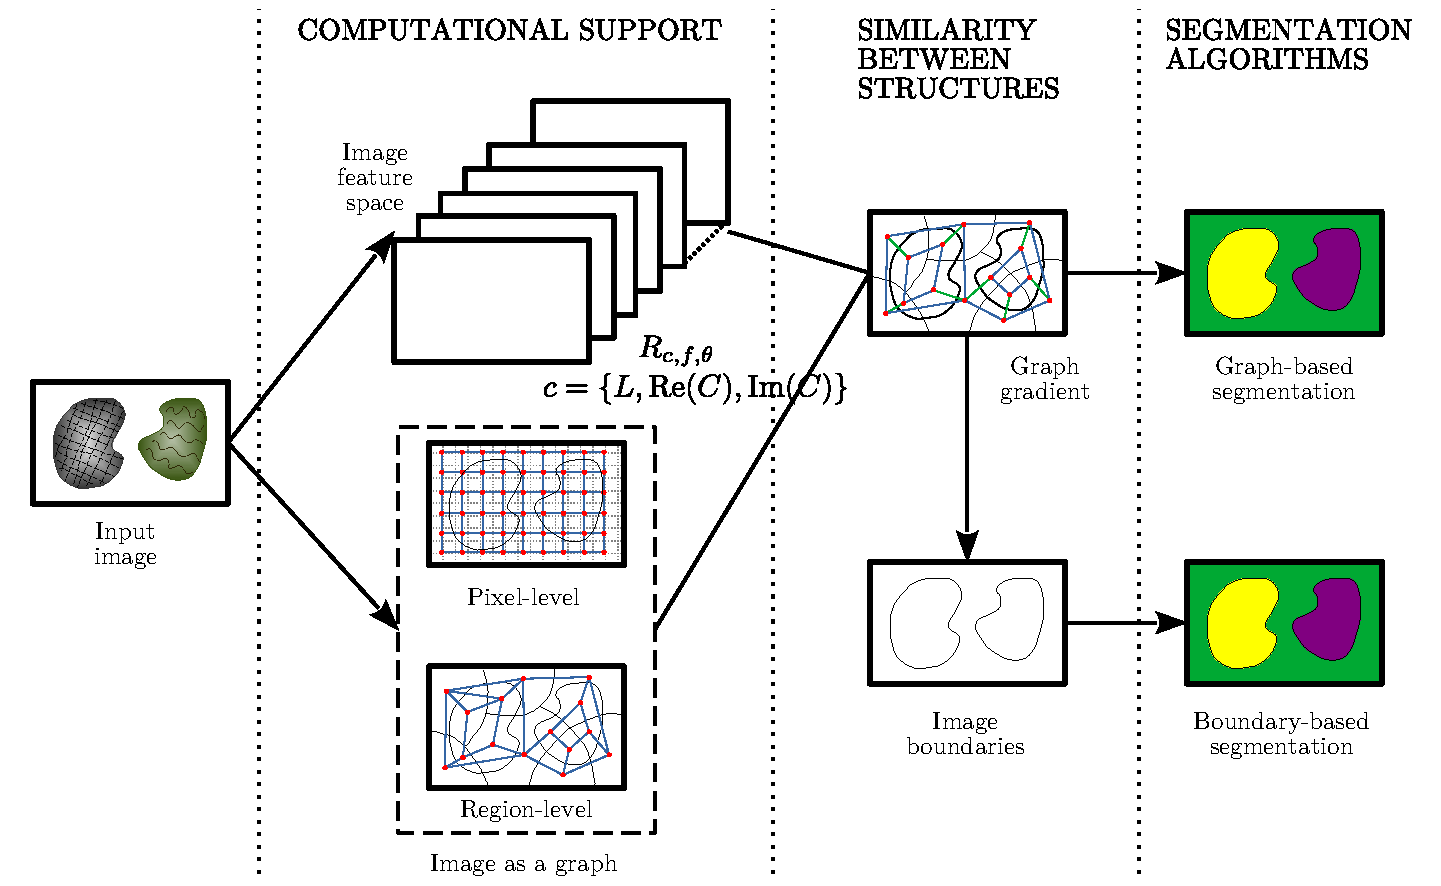
\includegraphics[width=\textwidth]{img_boundaries_segmentation_diagram}
	\caption{General pipeline for extraction of perceptual imagen boundaties and unsupervised image segmentation.}\label{fig:pipeline_gabor_image_segmentation}
\end{figure}

\section{Related work}
Edge detection is a fundamental problem of computer vision that has been intensively studied since the early 1970s \citep{Hueckel:JACM:1971, Fram.Deutsch:TC:1975}. The main idea behind traditional approaches to contour extraction is to model edges as discontinuities in the brightness channel of an image. This idea gave way to the creation of mask-based operators such as Sobel \citep{Maitre:Book:2003}, Roberts \citep{Roberts:Thesis:1963}, Gradient \citep{Maitre:Book:2003} and Prewitt \citep{Prewitt:PPP:1970}, which quantify the presence of an edge through the convolution of a gray level image with local derivative filters. Other techniques, such as Marr and Hildreth \citep{Marr.Hildreth:PRS:1980}, define edges as the zero crossings of the Laplacian of a Gaussian (LoG). Within traditional methods, the Canny \citep{Canny:PAMI:1986} operator is one of the most popular approaches to this day. This operator follows the same principle of operation of the previous methods, adding a non-maximum suppression stage and a hysteresis thresholding.

Despite their efficiency in controlled environments or in synthetic images, traditional methods suffer when it comes to identifying contours in natural images. The edges of natural images can be present at different scales, and the colors and textures of the scene can generate edges that are perceptually significant to the human eye. Ideally, a contour detection method is intended to simultaneously exploit the brightness, color and texture properties of an image in such a way that it can handle the boundary perimeters defined by the brightness steps and the regions with constant color and / or texture.

One of the relatively recent strategies for identifying perceptual contours is to use the local energy response of an image. The principle of operation is simple: generate features from the responses of an image produced by a family of filters at different scales and orientations. The idea has been exploited from different points of view. For example, the use of the  Difference of Gaussians (DoG) and its HIlbert transform \citep{Morrone.Owens:PR:1987, Morrone.Burr.ea:RSL:1988} for the generation of a family of filters. Inspired by Gabor's work, this group of filters comply with the Parseval principle; in addition to generating an exact quadrature pair (even and odd symmetry cells).

The \textit{Probability-of-boundary} (Pb) detector \citep{Malik.Belongie.ea:IJCV:2001} is one of the major exponents of the use of a filter bank formed by the DoG and its Hilbert transform. The contour detector only uses the brightness and texture information to obtain the Pb. The brightness information is processed following the intervening contour framework \citep{Leung.Malik:ECCV:1998} which consists in obtaining the quadrature energy of the image, also called oriented energy (OE). The texture information is analyzed using so-called textons \citep{Malik.Belongie.ea:ICCV:1999}. Since each cue (brightness and texture) has a domain of applicability, hence different units of magnitude, they introduce a gating operator based on the texturedness of a neighborhood at a pixel. The operator give as a result a local measure which indicates how much two nearby pixels are to belong to the same region. Later in that work, they use spectral graph theory (normalized cut algorithm \citep{JianboShi.Malik:PAMI:2000}) to segment the image into regions of coherent texture and brightness.

This contemporary method, developed by the UC Berkeley research group, was the basis for many other techniques for contour detection and segmentation of natural images widely used today. Most of these works bring substantial improvements to the Pb detector. For example, the seminal papers \citep{Martin.Fowlkes.ea:NIPS:2002} and \citep{Martin.Fowlkes.ea:PAMI:2004} bring together previous works related to Pb and obtain a feature space of four image characteristics: localized OE, Brightness Gradient (BG), Color Gradient (CG) and localized Texture Gradient (TG). To cope with the problem of the difference in units of magnitude of the cues, they use a logistic regression classifier to combine oriented energy, brightness, color and texture. The proposed supervised method optimizes the weights of each feature formulating it as a two-class classification problem, where they learn the rules for combining cues from the groundtruth data of the Berkeley Segmentation Dataset (BSDS) \citep{Martin.Fowlkes.ea:ICCV:2001}.

On the other hand, \cite{Ren:ECCV:2008} showed that the Pb detector improves when using features of the image calculated at different scales. However, a better version of the Pb detector, which has dominated the state of the art scores for several years, is obtained by combining local and global contours \citep{Maire.Arbelaez.ea:CVPR:2008}. The local contours are represented by the multiscale oriented signal mPb, while the global contours are represented by the oriented signal from the spectral partition sPb. The final detector that combines both signals is the globalized Probability-of-boundary gPb, which learns the weights of the local and global part by means of an ascending gradient, taking as reference the BSDS evaluation score.

The Berkeley research group laid the foundation for contour detection and natural image segmentation, providing tools for quantitative comparison of methods. However, there are other methods in the literature that use different strategies to calculate image features and detect contours. Such methods can use fully supervised approaches, avoiding the careful hand-drawing of texture and gloss gradients. However, we can also find semi-supervised methods that replace the Pb detector to later apply a preprocessing chain similar to that applied in the Berkeley group methods.

The Berkeley research group laid the foundation for contour detection and natural image segmentation, providing the database and tools for the comparison and quantitative evaluation of the different approaches. Furthermore, Pb has motivated the development of state-of-the-art methods that use totally different strategies to obtain image features and contour detection. Such methods can use fully supervised approaches, avoiding careful filter design, computation of texture and brightness gradients, and hand-crafted features. We can also find semi-supervised methods, which generally replace the Pb detector with a supervised detector to later apply a preprocessing chain similar to that applied in the Berkeley group methods to refine the detection.

The set of the most popular supervised methods for contour detection, led by researchers from the University of Pasadena California and colleagues, is based on the calculation of features on channels of integrals of the image \citep{Dollar.Tu.ea:BMVC:2009}. Some examples of these integral channels are: image color and gray channels, image responses to linear filters (e.g. Gabor filters, DoG), non-linear image transformations (e.g. Canny edges, gradient magnitude, hysteresis threshold), among others. The calculation of features on the integral channels follow the object detection framework of \cite{Viola.Jones:IJCV:2004}, obtaining first-order and higher-order features such as Haar-like features. Following this principle, a pool of features is obtained by randomly choosing both the integral channel and a rectangle on which the features are calculated, which allows the acceleration of the computation of features and the application of boosting techniques for learning.

Some of the supervised edge detectors that use the integral channel features as input are the Boosted Energy Learning (BEL) \citep{Dollar.ZhuowenTu.ea:CVPR:2006}, which attempts to learn an edge classifier in the form of a probabilistic boosting tree from the thousands of simple features calculated in image patches. On the other hand, Sketch tokens \citep{Lim.Zitnick.ea:CVPR:2013} uses the same features as input to a random forest classifier. The peculiarity of this second method is that the classes of the classifier are the so-called sketch tokens; mid-level information patches that represent complex shapes such as joints, corners, vertical and horizontal edges, etc., calculated from the contours of the groundtruth. The Structural Edge (SE) detector \citep{Dollar.Zitnick:ICCV:2013} and its different versions \citep{Dollar.Zitnick:PAMI:2015} take these strategies to another level, learning not only the integral input features but also the output space, using structured-output decision forests. The Oriented Edge Forest (OEF) detector \citep{Hallman.Fowlkes:CVPR:2015} outperforms existing supervised methods by using a decision forest that analyzes local patches and outputs probability distributions over the space of oriented edges passing through the patch. Finally, the detector based on a Deep Neural Network (DeepNet) architecture \citep{Kivinen.Williams.ea:PMLR:2014}, is a fully supervised method that does not use the integral features framework, instead, it calculates complex-cell like covariance features from multiple scales and semantic levels, which depend on the squared response of a filter to the input image.

Another group of approaches to contour detection are those based on local sparse coding. Such techniques are said semi-supervised because they contain two main stages, one unsupervised and the other supervised. The first stage consists of obtaining a generic representation (without information of the contours) from the information of the image in an unsupervised way. The second stage consists of transforming the sparse representation of the image into a specific labeling task, where in the case of contours detection is a two-classes supervised problem, which that lables the pixels as contour or no contour. Some renowned works under this approach are the detector proposed by \cite{Mairal.Leordeanu.ea:ECCV:2008} and the Sparse Code Gradients (SCG) detector \citep{Ren.Bo:NIPS:2012}. Both works use K-SVD as a dictionary learning algorithm and Orthogonal Matching Pursuit for efficient optimization and sparse coding of each pixel. At the end of the process, they use SVM as linear classifier on the feature vectors resulting from the reconstruction error with each dictionary for pixel classification. The main difference between these detectors is that the SCG adopts the same scheme as the Pb detector, replacing the brightness, color and texture gradients with sparse code gradients. Finally, the Sparse Code Transfer (SCT) detector \citep{Maire.Yu.ea:ACCV:2014} improves on the detector of \cite{Mairal.Leordeanu.ea:ECCV:2008} using a greater number of dictionaries at different scales and layers in addition to the multipath sparse coding technique, which rectifies the initial sparse codes to reconstruct the contours with an extra transfer dictionary. The main disadvantage of these semi-supervised methods is the computational time of both processes, dictionary calculation and learning.

There is a fine line between the contour detection and image segmentation. In this sense, the Pb contour detector has also had an influence on image segmentation. The Ultrametric Contour Maps (UCM) \citep{Arbelaez.Maire.ea:PR:2009} uses the gPb to define a measure of dissimilarity (ultrametric distance) between pairs of adjacent regions defined by a hierarchical segmentation operator (HSO). This technique is refined by adding a supplementary preprocessing stage using the oriented watershed transform (OWT), giving rise to the gPb-owt-ucm hierarchical segmentation method \citep{Arbelaez.Maire.ea:PR:2009}. The extensive qualitative and quantitative comparison of these techniques can be consulted in \citep{Arbelaez.Maire.ea:PAMI:2011}.

The Pb contour detector has driven (directly or indirectly) 50 years of research work around the detection of perceptual contours in natural images their segmentation. Like the Canny operator, the Pb operator has become the reference work. The importance of this method is that it provides a good basis that takes into account the principles of human perception, using operators that have a physical sense.


\begin{table}[]
\begin{tabular}{c|c|c|c}
\textbf{Edge detector} & \textbf{Input features}                                                                           & \textbf{Main approach}                                           & \textbf{\begin{tabular}[c]{@{}c@{}}Segmentation \\ technique\end{tabular}} \\ \hline
Pb                      & BG, TG                                                                                            & Gradients dissimilarity                                          & Normalized cuts                                                            \\
PMI                     & LUV color channels                                                                                & Pixel mutual information                                         & -                                                                          \\ \hline
SCG                     & \begin{tabular}[c]{@{}c@{}}Gray, color, and \\ depth channels\end{tabular}                        & \begin{tabular}[c]{@{}c@{}}Sparse coding\\ +\\ SVM\end{tabular}  & -                                                                          \\
SCT                     & RGB color channels                                                                                & \begin{tabular}[c]{@{}c@{}}Sparse coding\\  +\\ SVM\end{tabular} & -                                                                          \\ \hline
$\widehat{\text{Pb}}$   & BG, TG                                                                                            & Logistic regression                                              & Normalized cuts                                                            \\
gPb                     & $\widehat{\text{OE}}$, BG, CG, $\widehat{\text{TG}}$                                              & Logistic regression                                              & UCM + OWT                                                                  \\
BEL                     & Integral channel features                                                                         & Gradient boosting                                                & -                                                                          \\
Sketch tokens           & Integral channel features                                                                         & Random forest                                                    & -                                                                          \\
SE                      & Integral channel features                                                                         & Random forest                                                    & -                                                                          \\
OEF                     & Integral channel features                                                                         & Random forest                                                    & -                                                                          \\
DeepNet                  & Covariance-like features                                                                          & Deep NN                                                          & -                                                                          \\
ISCRA                   & \begin{tabular}[c]{@{}c@{}}BG, CG, TG, SIFT,\\  shape features, \\ boundary features\end{tabular} & Cascading classifier                                             & Region merging                                                             \\
COB                     & $\widehat{\text{OE}}$, BG, CG, $\widehat{\text{TG}}$                                              & Convolutional NN                                                 & -                                                                       
\end{tabular}
\end{table}

\section{Image as a graph}

Graphs are historical mathematical structures that have been applied to almost all fields of engineering. Historically, Euler made use of these structures to solve a problem related to the optimal crossing of people across bridges. The success of these structures in fields such as electricity and chemistry, contributed to the creation of a standard nomenclature, giving way to the Graph theory.

Fundamentally, a graph is an useful structure for modeling pairwise relations between objects. In this section, we present the notation and the commonly encountered graphs in image processing applications.


%In the field of image processing we can find several approaches that make use of graphs. Generally these methods solve a minimization problem. For example, the \textit{minimun spanning tree} approach that aims to find for each pair of nodes, the path with the least weight edges. On the other hand, the \textit{max-flow min-cut} approach aims to maximize flow with the minimum number of cuts in the graph. Both strategies have been successfully applied to the image segmentation problem. Another application example involves the algebraic theory of graphs that studies the spectrum of matrices that represent graphs.



\subsection{Graph notations and definitions}

In this section we introduce some important definitions that will be used throughout the chapter related to graphs and some related structures.

\theoremstyle{definition}
\begin{definition}[Graph]
	A graph $\mathcal{G}$ is defined by the finite sets $(\mathsf{V}, \mathsf{E})$ in which $\mathsf{E} \subset \mathsf{V} \times \mathsf{V}$. The elements of $\mathsf{v} \in \mathsf{V}$ are called \textit{vertices} and the elements of $\mathsf{e} \in \mathsf{E}$ are called edges. Since the edges are a subset of two nodes, we can write them as $\mathsf{e}_{i,j}$, $\{i, j\}$ or $\{\mathsf{v}_{i}, \mathsf{v}_{j}\} \quad \forall i, j \in \mathsf{V}$.
\end{definition}

\begin{definition}[Neighborhood]
	A neighborhood is a set of adjacent vertices to a vertex $\mathsf{v}_i$ and is denoteb by $N_i = \{\mathsf{v}_j \in \mathsf{V}  | \exists d(\mathsf{v}_i, \mathsf{v}_j)\}$, where $d(\mathsf{v}_i, \mathsf{v}_j)$ defines a distance function between vertices.
\end{definition}

\begin{definition}[Subgraph]
	A subgraph $\mathcal{G}'= (\mathsf{V}', \mathsf{E}')$ is a (partial) graph of $\mathcal{G}=(\mathsf{V}, \mathsf{E})$ if $\mathsf{V}' \subseteq \mathsf{V}$, and  $\mathsf{E}'= \{\mathsf{e}_{i,j} \in \mathsf{E} | \mathsf{v}_i \in \mathsf{V}' \}$.
\end{definition}

\begin{definition}[Edge-weighted graph]
	Given a graph $\mathcal{G}=(\mathsf{V}, \mathsf{E})$, egde weighting is a function $\omega: \mathsf{E} \rightarrow \mathbb{R}$. The weight of an edge incident to two vertices is denoted by  $\omega(\mathsf{v}_{i}, \mathsf{v}_{j})$, $ \omega(\mathsf{e}_{i,j})$ or simply as $\omega_{i,j}$.
\end{definition}

\begin{definition}[Node-weighted graph]
	Given a graph $\mathcal{G}=(\mathsf{V}, \mathsf{E})$, vertex weighting is a function $\hat{\omega}: \mathsf{V} \rightarrow \mathbb{R}$. The weight of a vertex is denoted by  $\hat{\omega}(\mathsf{v}_{i})$ or simply as $\hat{\omega}_{i}$.
\end{definition}

\begin{definition}[Adjacency]
	Given an edge $\mathsf{e}_{i,j}$ that connects $\{\mathsf{v}_{i}, \mathsf{v}_{j}\} $, the two vertices $\{\mathsf{v}_{i}, \mathsf{v}_{j}\}$ contained in the edge are said to be \textit{adjacent} or \textit{neighbors}. In the same way two edges that share a vertex are \textit{adjacent}.
\end{definition}

\begin{definition}[Adjacency matrix]
	The adjacency matrix of a graph $\mathcal{G}=(\mathsf{V}, \mathsf{E})$ is a $|\mathsf{V}| \times |\mathsf{V}|$ matrix $A_{\mathcal{G}}$ that indicates whether pairs of vertices are adjacent or not. For undirected graphs, it is a symmetric $(0,1)$-matrix with zeros on its diagonal such that 
	
	\begin{equation}	
		A_{\mathcal{G}} = (a_{ij})_{(i, j)\in \{1,\cdots, n\}}  \quad \text{where $n$ is the number of nodes in $\mathcal{G}$ and} \nonumber 		
	\end{equation}
	\begin{equation}	
		a_{ij}= 
		\begin{cases}
			1 \quad \text{if $i, j$ are adjacent in $\mathcal{G}$} \\
			0 \quad \text{elsewhere}
		\end{cases}		\nonumber		
	\end{equation}
\end{definition}


%{Wang.Liu.ea:SP:2017} reference about superpixel benchmark

\subsubsection{Pixel-based graph representation}

Considering a digital image as a 2-d grid of pixels, where the intensity (or color) values are mapped to the spatial coordinates $(x, y)$, we can use the graph theory to represent all the pixels as a dense graph. In terms of a graph $\mathcal{G}=(\mathsf{V}, \mathsf{E})$, each node $\mathsf{v}_i \in \mathsf{V}$ corresponds to a pixel in the image, and edges link the pixels of the image. 

There are several strategies to join the nodes of a graph. The types of graphs that we can form are a function of such union strategies. For example, the complete graph connects each pair of different nodes with a single edge. The epsilon-graph connects a pair of nodes if they are within an epsilon distance. The k-nearest neighbors graph (knn-graph) connects a central node to another node only if the distance between them is among the k smallest distances from the central node to other nodes. Lastly, the adjacency graph connects only a pair of nodes if they are neighbors or adjacent. At a pixel level, this last graph is referred to as \textit{pixel adjacency graph} (PAG).

We can define the adjacency level of the pixels to generate a specific pixel-based graph. In our applications we mainly use the 4-neighbor adjacency system. This and other adjacency systems based are illustrated in figure \ref{fig:pixel_adjacency_graph}.


\begin{figure}[!ht]
    \centering

	\begin{subfigure}[b]{0.2\textwidth}
    	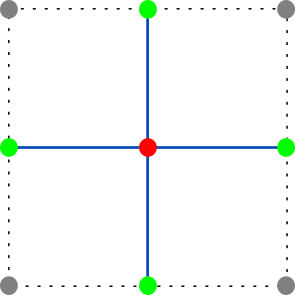
\includegraphics[width=\textwidth]{4nn_pag}
        \caption{ 4-neighborhood}
    \end{subfigure}\qquad   
    \begin{subfigure}[b]{0.2\textwidth}
    	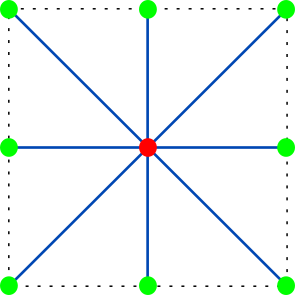
\includegraphics[width=\textwidth]{8nn_pag}
        \caption{8-neighborhood}
    \end{subfigure}\qquad
    \begin{subfigure}[b]{0.23\textwidth}
    	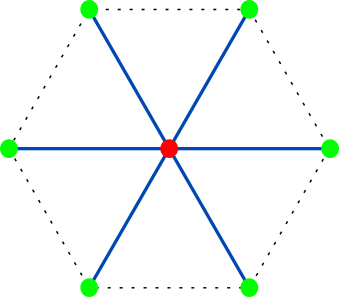
\includegraphics[width=\textwidth]{6nn_pag}
        \caption{6-neighborhood}
    \end{subfigure}\\[5ex]    
    \begin{subfigure}[b]{0.5\textwidth}
        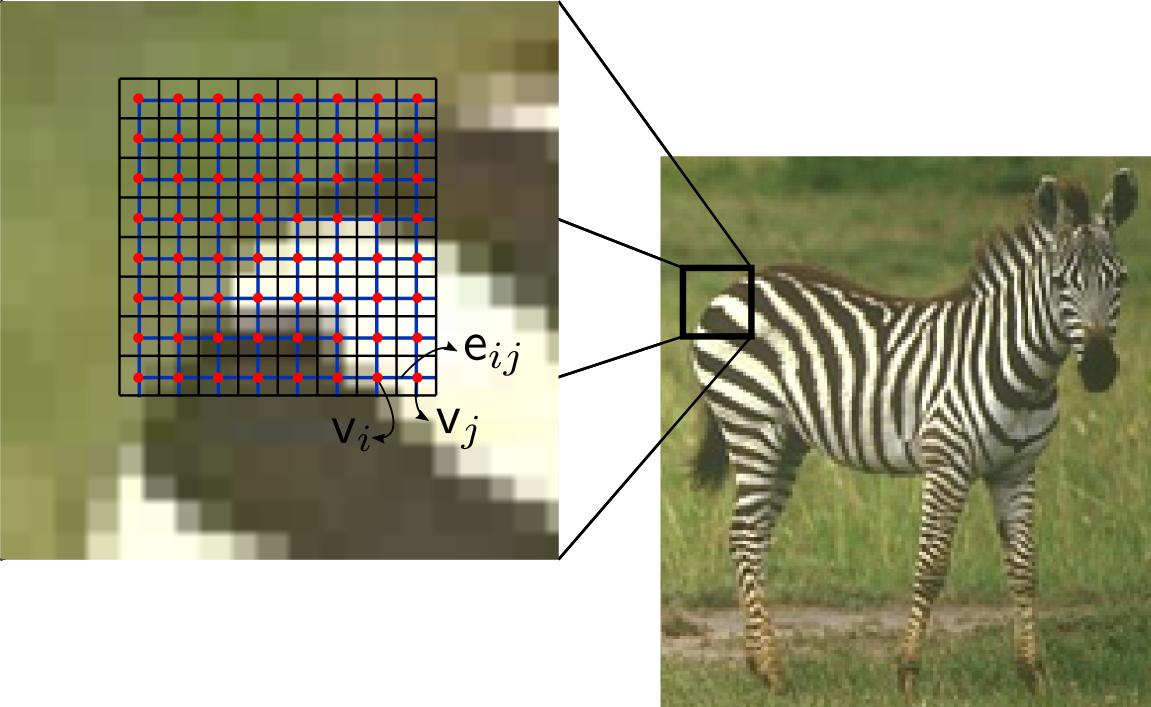
\includegraphics[width=\textwidth]{pixel_adjacency_graph}
        \caption{Exaple of a 4-n graph on a real image}
    \end{subfigure}         
        	    
    \caption{Most common k-nearest neighbors adjacency systems.}\label{fig:pixel_adjacency_graph}    
\end{figure}

The representation of an image as a graph opens the possibility of new methods for data processing, however, a recurring problem is the need to satisfy the compromise between algorithmic complexity and precision of the methods. In most algorithms, complexity is a function of the number of nodes and edges in the graph, so the adjacency system used plays an important role in the speed of the methods applied to image graph. One way to reduce the number of nodes (and consequently the number of edges) is to use graphs on elements or regions of the image of greater size.

\subsubsection{Region-based graph representation}

To build this type of graph, we must first separate the image into regions, preferably into regions that are coherent with the perceptual information of the image. Subsequently, the nodes of a graph represent the regions of the image while the egdes follow the same strategies described above to connect the regions. The main type of graph that we consider in this work is the \textit{region adjacency graph }(RAG).


\begin{figure}[!ht]
	\centering
	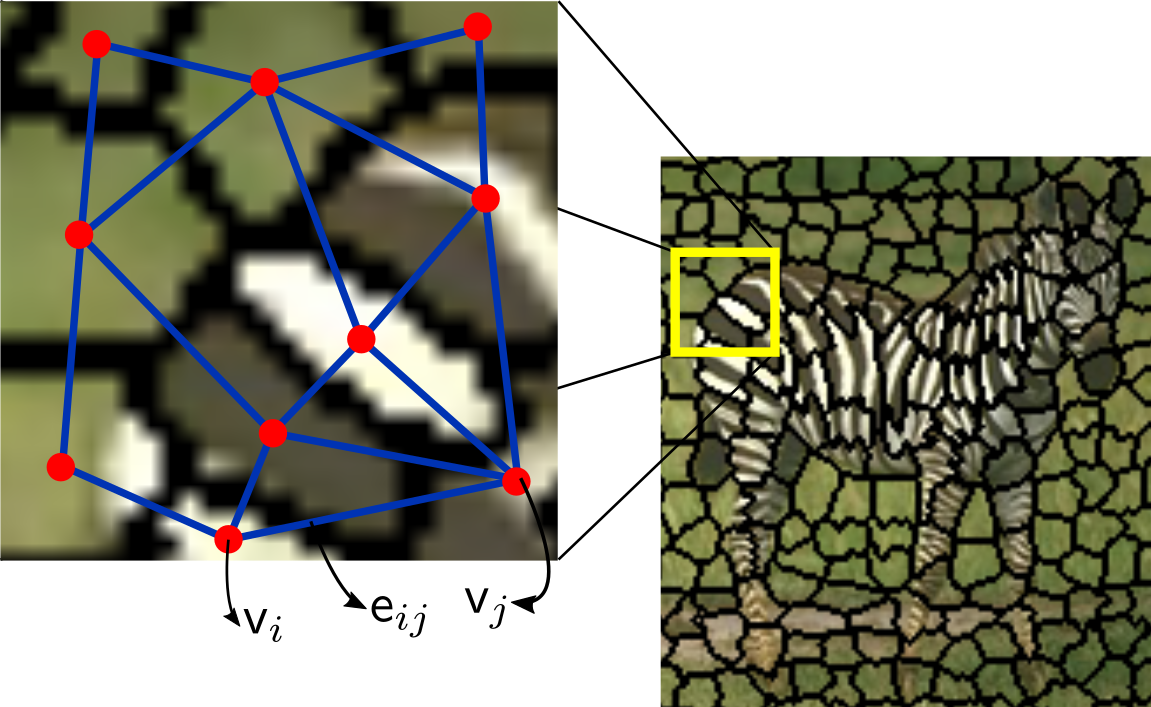
\includegraphics[width=0.5\textwidth]{region_adjacency_graph}       	    
    \caption{Exaple of a Region Adjacency Graph on a real image.}\label{fig:region_adjacency_graph}    
\end{figure}


Pixels are the smallest elements in the image. The grouping of these elements in coherent regions generates so-called superpixels. In the next section we introduce some of the most used methods for the generation of these regions, exposing their main characteristics.


\subsection{Superpixels}

Pixels are a consequence of the discrete representation of the intensity or color of an image, therefore pixels are not entities that naturally reflect the perceptual information in an image. Moreover, the number of pixels on an image is to high (even in moderate resolutions) making the optimization at pixel level difficult. The superpixels are local coherent and preserve most of the stucture necessary for image processing algorithms.

The term \textit{superpixels} was introduced first by \cite{Ren.Malik:ICCV:2003} to describe the resulting regions of an oversegmentation image process. However, \cite{Stutz.Hermans.ea:CVIU:2018} gathers a series of requirements from different works of the state of the art to differentiate superpixels from other regions generated by over-segmentation algorithms. 

\begin{itemize}
 \item \textbf{Partition}. Superpixels should define a partition of the image. They should be disjoint and assign a label to every pixel.
 \item \textbf{Connectivity}. Superpixels represents a connected set of pixels.
 \item Boundary Adherence. Superpixels must preserve image bundaries.
 \item \textbf{Compactness, Regularity and Smoothness}. Superpixels should be compact (closed and bounded), placed regulary and exibit smooth boundaries.
 \item \textbf{Efficiency}. Shuold be generated efficiently
 \item \textbf{Controllable number of superpixels}. The number of superpixels should be controllable.
\end{itemize}

In addition, according to the followed strategy   to obtain the regions, \cite{Stutz.Hermans.ea:CVIU:2018} propouse a classification for superpixels techniques. We present here four super pixel techniques; each one of them representative of a category the classification. 


%\begin{enumerate}
% \item \textbf{Watershed-based.} Based on the watershed algorithm, these methods generally depends on a image pre-processing step and the markers setting. 
% \item \textbf{Density-based.} Perform mode-seeking in a computed density image. These methods usually do not offer control over the number of superpixels or their compactness (they are consider as oversegmentation algorithms). 
% \item \textbf{Graph-based.} Treat the image as undirected graph and do a the image partition based on edge-weights  (computed as color differences or similarities).
% \item \textbf{Clustering-based.} Inspired in clissical clustering methods (k-means), these techniques group the pixels from seed pixels using color information, spacial information, and other (such as depth information). The number of superpixels and their compactness is controllable.
%\end{enumerate}


\subsubsection{Felzenszwalb's Superpixels}

This technique belongs to the category of graph-based superpixels, which represent the region generation problem in terms of an edge-weighted undirected graph. 

Treat the image as undirected graph and do a the image partition based on edge-weights  (computed as color differences or similarities). The weight of an edge  $\omega_{ij}$
can be obtained in two ways,
\begin{enumerate}
	\item $\omega(\mathsf{v}_i, \mathsf{v}_j)= I(p_i) - I(p_j)|$, the absolute intensity difference between the pixels connected by an edge; 
	\item $\omega(\mathsf{v}_i, \mathsf{v}_j)= X(p_i) - X(p_j)|$, the L2 (Euclidean)
distance between two corresponding pixels in feature space.
\end{enumerate}

For color images is possible to use the option 1 considering each color channel as a individual intensity channel and then combine the tree weights. Otherwise, the feature space of option 2 is defined by $X = (x, y,r, g, b)$, where $(x, y)$ is the location of the pixels in the image and $(r, g, b)$ is the color value of the pixels. This method uses a Gaussian filter to smooth the image before the edge weights computation to compensate for digitization artifacts. 

Whit this method we cannot directly control the number of resulting superpixels, we must use the Gaussian scale parameter to modify the size and shape of the superpixels. However, the actual size and number of segments can vary greatly, depending on local contrast.

\begin{figure}[!ht]
    \centering
    \begin{subfigure}[t]{\dimexpr0.2\textwidth+20pt\relax}
    	\makebox[20pt]{\raisebox{25pt}{ \rotatebox[origin=c]{90} {\small \textsf{\textbf{Input image}}} }}%
    	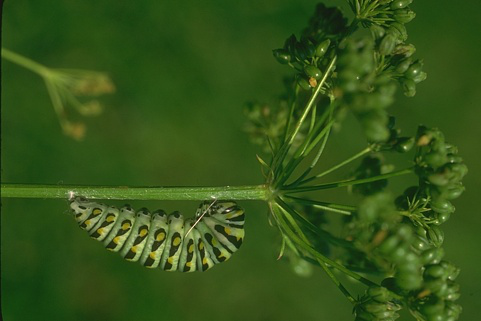
\includegraphics[width=\dimexpr\linewidth-20pt\relax]{35028} 
    \end{subfigure}      
    ~ %add desired spacing between images, e. g. ~, \quad, \qquad, \hfill etc. 
      %(or a blank line to force the subfigure onto a new line)
    \begin{subfigure}[b]{0.2\textwidth}
        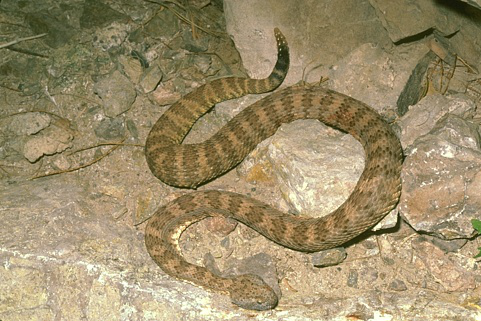
\includegraphics[width=\textwidth]{87015}
    \end{subfigure}
    ~ %add desired spacing between images, e. g. ~, \quad, \qquad, \hfill etc. 
      %(or a blank line to force the subfigure onto a new line)
    \begin{subfigure}[b]{0.2\textwidth}
        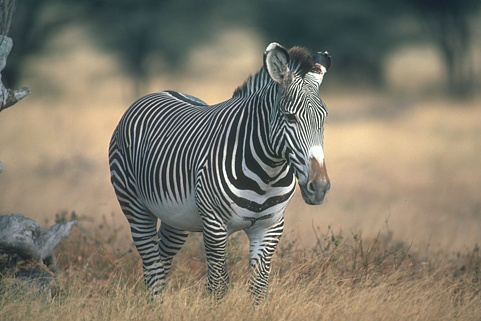
\includegraphics[width=\textwidth]{130066}
    \end{subfigure}
    ~ %add desired spacing between images, e. g. ~, \quad, \qquad, \hfill etc. 
      %(or a blank line to force the subfigure onto a new line)
    \begin{subfigure}[b]{0.2\textwidth}
        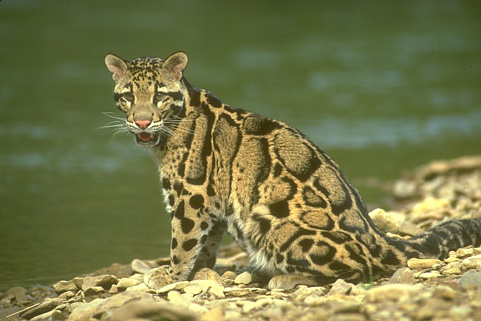
\includegraphics[width=\textwidth]{160067}
    \end{subfigure} \\[2ex]       
    
    \begin{subfigure}[t]{\dimexpr0.2\textwidth+20pt\relax}
    	\makebox[20pt]{\raisebox{25pt}{ \rotatebox[origin=c]{90} {\small \textsf{\textbf{150 sp}}} }}%
    	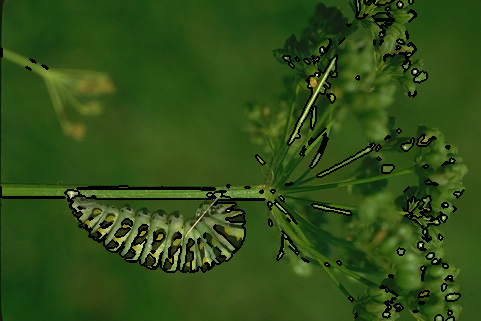
\includegraphics[width=\dimexpr\linewidth-20pt\relax]{35028_fz_150_segs} 
    \end{subfigure}      
    ~ %add desired spacing between images, e. g. ~, \quad, \qquad, \hfill etc. 
      %(or a blank line to force the subfigure onto a new line)
    \begin{subfigure}[b]{0.2\textwidth}
        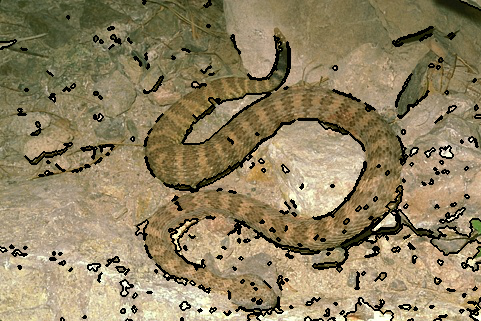
\includegraphics[width=\textwidth]{87015_fz_150_segs}
    \end{subfigure}
    ~ %add desired spacing between images, e. g. ~, \quad, \qquad, \hfill etc. 
      %(or a blank line to force the subfigure onto a new line)
    \begin{subfigure}[b]{0.2\textwidth}
        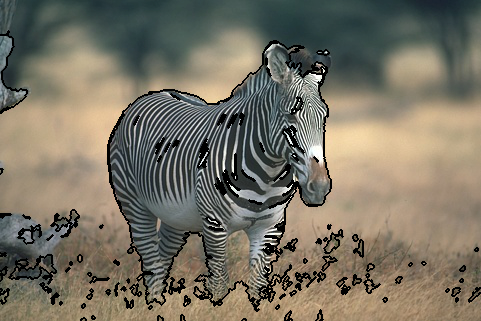
\includegraphics[width=\textwidth]{130066_fz_150_segs}
    \end{subfigure}
    ~ %add desired spacing between images, e. g. ~, \quad, \qquad, \hfill etc. 
      %(or a blank line to force the subfigure onto a new line)
    \begin{subfigure}[b]{0.2\textwidth}
        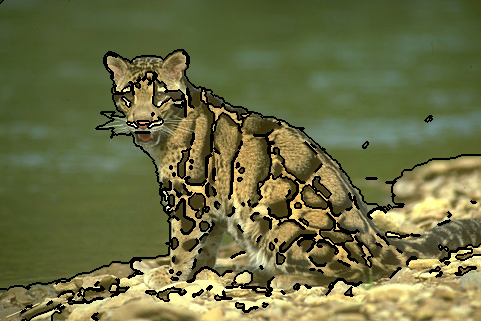
\includegraphics[width=\textwidth]{160067_fz_150_segs}
    \end{subfigure} \\ [2ex]
    
    \begin{subfigure}[t]{\dimexpr0.2\textwidth+20pt\relax}
    	\makebox[20pt]{\raisebox{25pt}{ \rotatebox[origin=c]{90} {\small \textsf{\textbf{300 sp}}} }}%
    	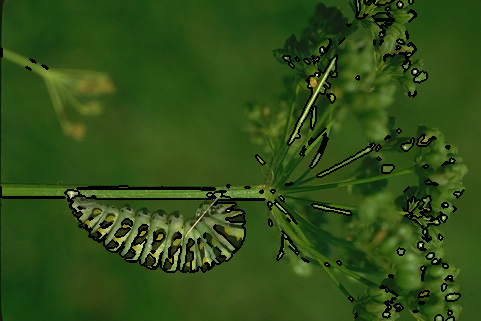
\includegraphics[width=\dimexpr\linewidth-20pt\relax]{35028_fz_150_segs} 
    \end{subfigure}      
    ~ %add desired spacing between images, e. g. ~, \quad, \qquad, \hfill etc. 
      %(or a blank line to force the subfigure onto a new line)
    \begin{subfigure}[b]{0.2\textwidth}
        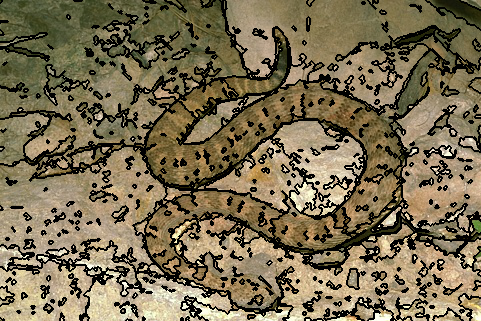
\includegraphics[width=\textwidth]{87015_fz_300_segs}
    \end{subfigure}
    ~ %add desired spacing between images, e. g. ~, \quad, \qquad, \hfill etc. 
      %(or a blank line to force the subfigure onto a new line)
    \begin{subfigure}[b]{0.2\textwidth}
        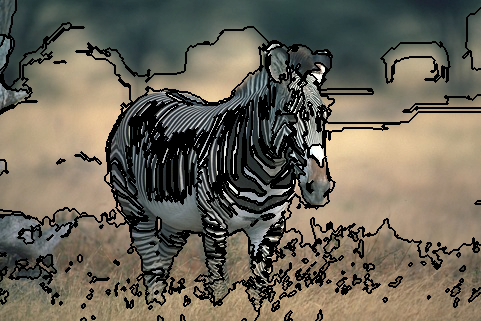
\includegraphics[width=\textwidth]{130066_fz_300_segs}
    \end{subfigure}
    ~ %add desired spacing between images, e. g. ~, \quad, \qquad, \hfill etc. 
      %(or a blank line to force the subfigure onto a new line)
    \begin{subfigure}[b]{0.2\textwidth}
        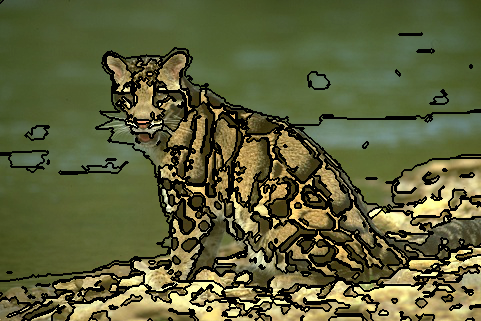
\includegraphics[width=\textwidth]{160067_fz_300_segs}
    \end{subfigure} \\ [2ex]
    
    \begin{subfigure}[t]{\dimexpr0.2\textwidth+20pt\relax}
    	\makebox[20pt]{\raisebox{25pt}{ \rotatebox[origin=c]{90} {\small \textsf{\textbf{600 sp}}} }}%
    	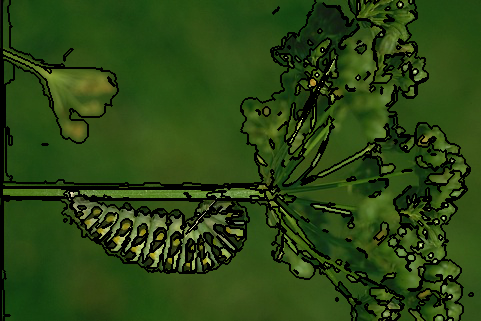
\includegraphics[width=\dimexpr\linewidth-20pt\relax]{35028_fz_600_segs} 
    \end{subfigure}      
    ~ %add desired spacing between images, e. g. ~, \quad, \qquad, \hfill etc. 
      %(or a blank line to force the subfigure onto a new line)
    \begin{subfigure}[b]{0.2\textwidth}
        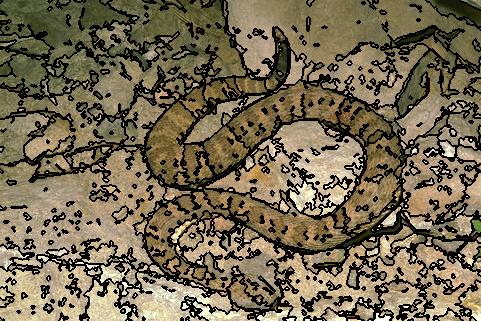
\includegraphics[width=\textwidth]{87015_fz_600_segs}
    \end{subfigure}
    ~ %add desired spacing between images, e. g. ~, \quad, \qquad, \hfill etc. 
      %(or a blank line to force the subfigure onto a new line)
    \begin{subfigure}[b]{0.2\textwidth}
        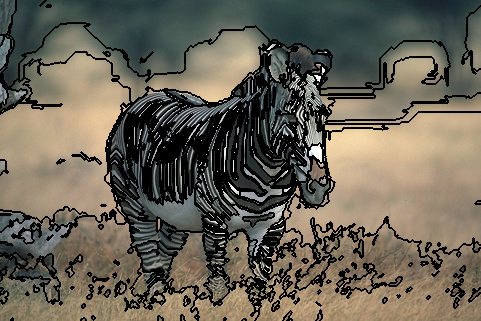
\includegraphics[width=\textwidth]{130066_fz_600_segs}
    \end{subfigure}
    ~ %add desired spacing between images, e. g. ~, \quad, \qquad, \hfill etc. 
      %(or a blank line to force the subfigure onto a new line)
    \begin{subfigure}[b]{0.2\textwidth}
        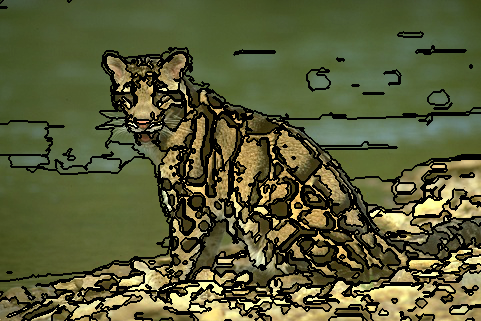
\includegraphics[width=\textwidth]{160067_fz_600_segs}
    \end{subfigure}     

	\caption{Examples of superpixels using Felzenszwalb's technique.}\label{fig:fz_suprepixels}    
\end{figure}

Figure \ref{fig:fz_suprepixels} shows the superpixels generated adjusting the scale parameter to obtain approximately 150, 300 and 600 super pixels (sp). The examples show that Felzenszwalb's superpixel technique acts more like an over-segmentation algorithm since neither the size nor the shape of the regions are close to being homogeneous. 
 
%In the graph-based approach, a segmentation $S$ is a partition of $V$ into components such that each component (or region) $C \in S$ corresponds to a connected component in a graph $G = (V, E)$, where $E \subseteq E$. In other words, any segmentation is induced by a subset of the edges in $E$. There are different ways to measure the quality of a segmentation but in general we want the elements in a component to be similar, and elements in different components to be dissimilar. This means that edges between two vertices in the same component should have relatively low weights, and edges between vertices in different components should have higher weights.

\subsubsection{Quick shift superpixels} %and kernel methods for mode seeking

The Quick Shift \citep{Vedaldi.Soatto:ECCV:2008} is a density-based method for superpixel computation. This technique perform a so-called mode-seeking algorithm \citep{YizongCheng:PAMI:1995} for locating the maxima of a density function. That is, it locates the maxima or the modes of a density function given discrete data sampled from that function through a mean shift procedure.

This is an iterative method that cannot offer control over the number of superpixels or their compactness and are, therefore, also categorized as an oversegmentation algorithm.

Quickshift computer a hierarchical segmentation of the image at multiple scales simultaneously. Then the parameters to define the size and shape of the regions depend on the scale of the local density approximation and the level in the hierarchical segmentation that is produced. Additionally, the compromise between color space and distance in image space can also be controlled. 

\begin{figure}[!ht]
    \centering
    \begin{subfigure}[t]{\dimexpr0.2\textwidth+20pt\relax}
    	\makebox[20pt]{\raisebox{25pt}{ \rotatebox[origin=c]{90} {\small \textsf{\textbf{Input image}}} }}%
    	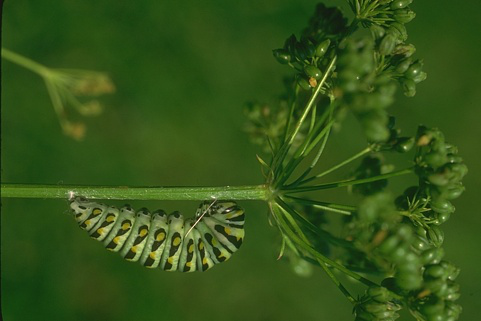
\includegraphics[width=\dimexpr\linewidth-20pt\relax]{35028} 
    \end{subfigure}      
    ~ %add desired spacing between images, e. g. ~, \quad, \qquad, \hfill etc. 
      %(or a blank line to force the subfigure onto a new line)
    \begin{subfigure}[b]{0.2\textwidth}
        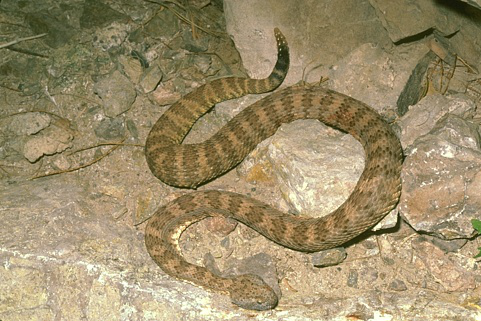
\includegraphics[width=\textwidth]{87015}
    \end{subfigure}
    ~ %add desired spacing between images, e. g. ~, \quad, \qquad, \hfill etc. 
      %(or a blank line to force the subfigure onto a new line)
    \begin{subfigure}[b]{0.2\textwidth}
        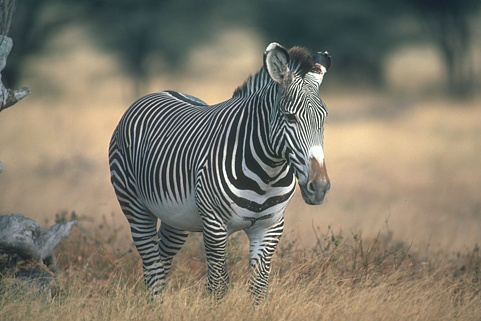
\includegraphics[width=\textwidth]{130066}
    \end{subfigure}
    ~ %add desired spacing between images, e. g. ~, \quad, \qquad, \hfill etc. 
      %(or a blank line to force the subfigure onto a new line)
    \begin{subfigure}[b]{0.2\textwidth}
        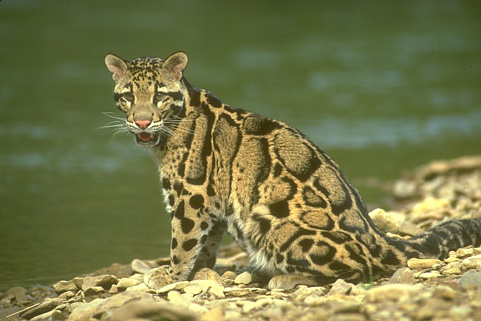
\includegraphics[width=\textwidth]{160067}
    \end{subfigure} \\[2ex]       
    
    \begin{subfigure}[t]{\dimexpr0.2\textwidth+20pt\relax}
    	\makebox[20pt]{\raisebox{25pt}{ \rotatebox[origin=c]{90} {\small \textsf{\textbf{150 sp}}} }}%
    	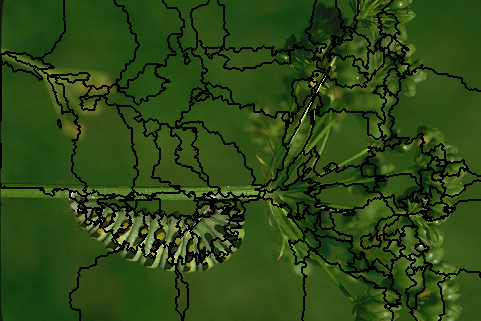
\includegraphics[width=\dimexpr\linewidth-20pt\relax]{35028_quick_150_segs} 
    \end{subfigure}      
    ~ %add desired spacing between images, e. g. ~, \quad, \qquad, \hfill etc. 
      %(or a blank line to force the subfigure onto a new line)
    \begin{subfigure}[b]{0.2\textwidth}
        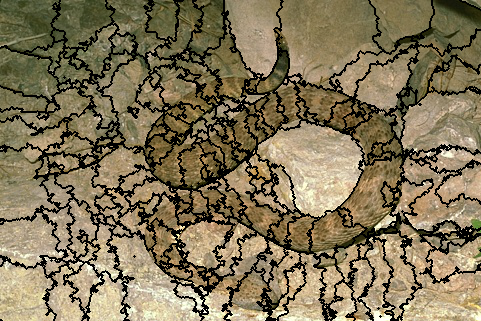
\includegraphics[width=\textwidth]{87015_quick_150_segs}
    \end{subfigure}
    ~ %add desired spacing between images, e. g. ~, \quad, \qquad, \hfill etc. 
      %(or a blank line to force the subfigure onto a new line)
    \begin{subfigure}[b]{0.2\textwidth}
        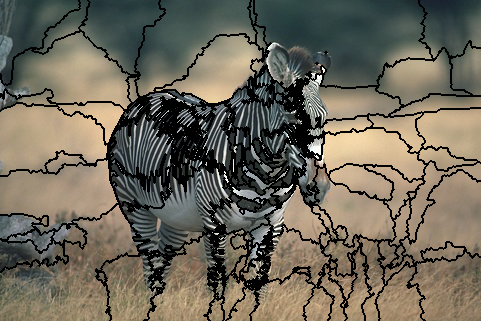
\includegraphics[width=\textwidth]{130066_quick_150_segs}
    \end{subfigure}
    ~ %add desired spacing between images, e. g. ~, \quad, \qquad, \hfill etc. 
      %(or a blank line to force the subfigure onto a new line)
    \begin{subfigure}[b]{0.2\textwidth}
        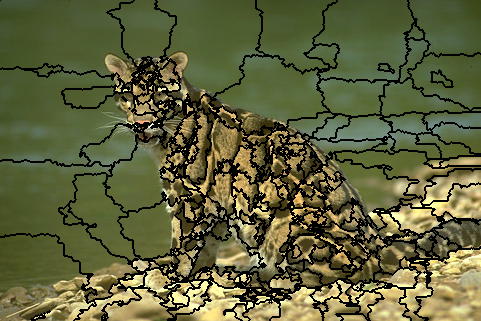
\includegraphics[width=\textwidth]{160067_quick_150_segs}
    \end{subfigure} \\ [2ex]
    
    \begin{subfigure}[t]{\dimexpr0.2\textwidth+20pt\relax}
    	\makebox[20pt]{\raisebox{25pt}{ \rotatebox[origin=c]{90} {\small \textsf{\textbf{300 sp}}} }}%
    	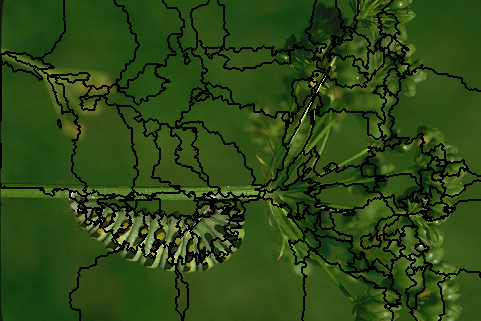
\includegraphics[width=\dimexpr\linewidth-20pt\relax]{35028_quick_150_segs} 
    \end{subfigure}      
    ~ %add desired spacing between images, e. g. ~, \quad, \qquad, \hfill etc. 
      %(or a blank line to force the subfigure onto a new line)
    \begin{subfigure}[b]{0.2\textwidth}
        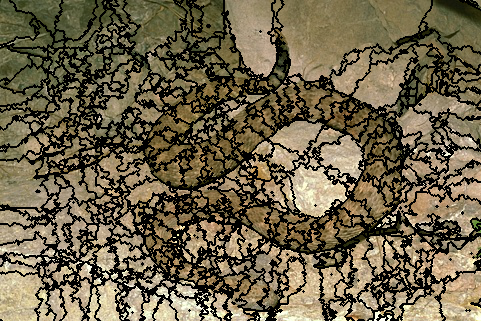
\includegraphics[width=\textwidth]{87015_quick_300_segs}
    \end{subfigure}
    ~ %add desired spacing between images, e. g. ~, \quad, \qquad, \hfill etc. 
      %(or a blank line to force the subfigure onto a new line)
    \begin{subfigure}[b]{0.2\textwidth}
        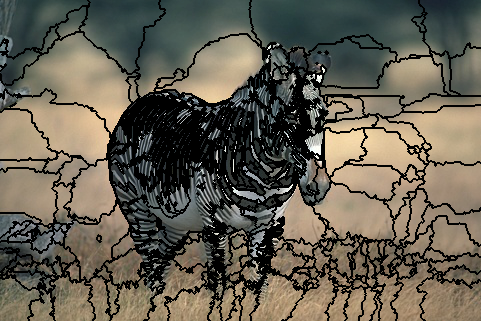
\includegraphics[width=\textwidth]{130066_quick_300_segs}
    \end{subfigure}
    ~ %add desired spacing between images, e. g. ~, \quad, \qquad, \hfill etc. 
      %(or a blank line to force the subfigure onto a new line)
    \begin{subfigure}[b]{0.2\textwidth}
        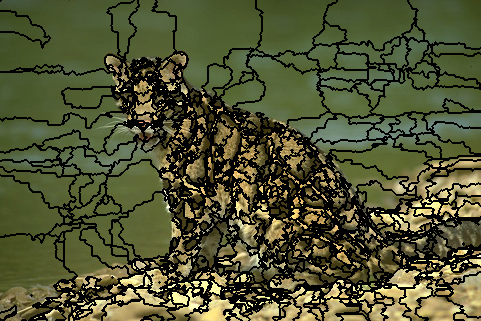
\includegraphics[width=\textwidth]{160067_quick_300_segs}
    \end{subfigure} \\ [2ex]
    
    \begin{subfigure}[t]{\dimexpr0.2\textwidth+20pt\relax}
    	\makebox[20pt]{\raisebox{25pt}{ \rotatebox[origin=c]{90} {\small \textsf{\textbf{600 sp}}} }}%
    	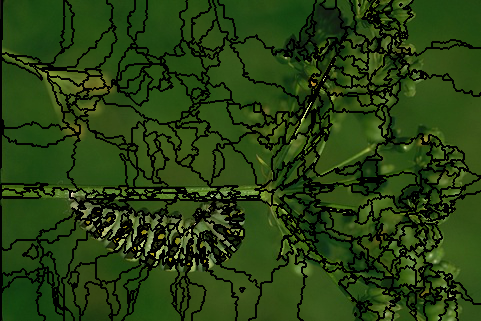
\includegraphics[width=\dimexpr\linewidth-20pt\relax]{35028_quick_600_segs} 
    \end{subfigure}      
    ~ %add desired spacing between images, e. g. ~, \quad, \qquad, \hfill etc. 
      %(or a blank line to force the subfigure onto a new line)
    \begin{subfigure}[b]{0.2\textwidth}
        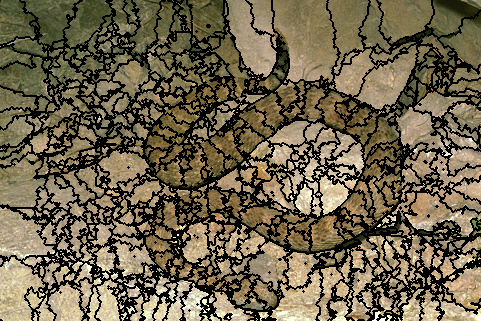
\includegraphics[width=\textwidth]{87015_quick_600_segs}
    \end{subfigure}
    ~ %add desired spacing between images, e. g. ~, \quad, \qquad, \hfill etc. 
      %(or a blank line to force the subfigure onto a new line)
    \begin{subfigure}[b]{0.2\textwidth}
        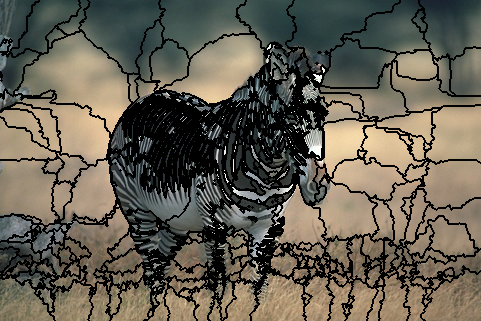
\includegraphics[width=\textwidth]{130066_quick_600_segs}
    \end{subfigure}
    ~ %add desired spacing between images, e. g. ~, \quad, \qquad, \hfill etc. 
      %(or a blank line to force the subfigure onto a new line)
    \begin{subfigure}[b]{0.2\textwidth}
        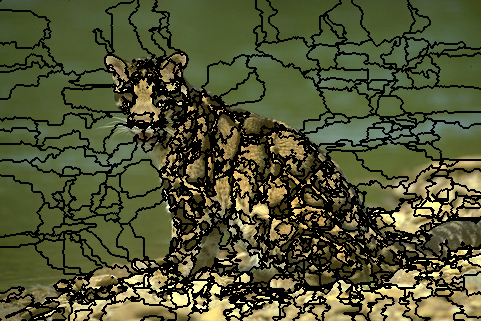
\includegraphics[width=\textwidth]{160067_quick_600_segs}
    \end{subfigure}     

	\caption{Eamples of Quick Shift superpixels.}\label{fig:quick_suprepixels}    
\end{figure}

We illustrate in figure \ref{fig:quick_suprepixels} four images and the superpixels obtained with the quickshift algorithm setting the parameters to obtain 150, 300 and 600 super pixels. 


\subsubsection{Watershed superpixels}%Compact watershed segmentation of gradient images
The watershed-based superpixel techniques takes the watershed segmentation algortihm proposed by \citep{Meyer:ICIP:1992} as calculation basis. Originally, the watershed method is an over segmentation technique, i.e., one can control the number of regions by means of the number of markers but we cannot control its compactness.  In this context, high compactness means that the superpixels are of approximately equal size and more or less regularly shaped in the absence of strong image gradients (e.g. like a recangle or a circle). Some watershed-based superpixel algorithms, such as the Compact watershed algortihm \citep{Neubert.Protzel:ICPR:2014} or the Water Pixels algorithm \citep{Machairas.Faessel.ea:IP:2015}, upgrades the original algorithm adding the compactness. 

Initially, these algorithms implements a seeded watershed segmentation (also called marker controlled watershed). Markers can be determined manually, or automatically using for example the local minima of the gradient of the image, or the local maxima of the distance function to the background. Therefore, instead of taking a color image as input, watershed requires a grayscale gradient image, where bright pixels denote a boundary between regions. 

Once the markers and the gradient are given, the algorithm views the image as a landscape, where bright pixels of the gradeint forms high peaks. This landscape is then flooded from the given markers, until separate flood basins meet at the peaks. Each distinct basin forms a different image segment.

The figure \ref{fig:wt_suprepixels} shows the superpixels obtained with the compact watershed algorithm \citep{Neubert.Protzel:ICPR:2014} defining the number of superpixels to find at 150, 300 and 600.


\begin{figure}[!ht]
    \centering
    \begin{subfigure}[t]{\dimexpr0.2\textwidth+20pt\relax}
    	\makebox[20pt]{\raisebox{25pt}{ \rotatebox[origin=c]{90} {\small \textsf{\textbf{Input image}}} }}%
    	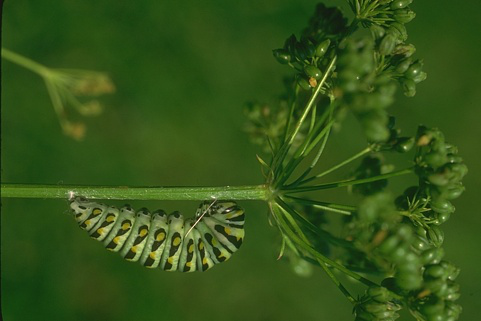
\includegraphics[width=\dimexpr\linewidth-20pt\relax]{35028} 
    \end{subfigure}      
    ~ %add desired spacing between images, e. g. ~, \quad, \qquad, \hfill etc. 
      %(or a blank line to force the subfigure onto a new line)
    \begin{subfigure}[b]{0.2\textwidth}
        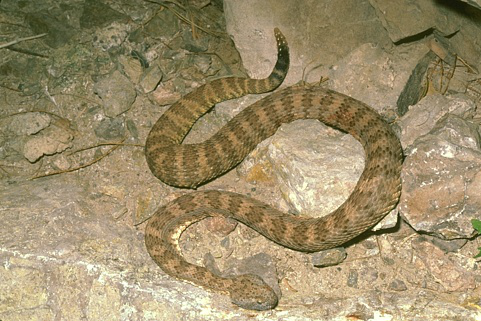
\includegraphics[width=\textwidth]{87015}
    \end{subfigure}
    ~ %add desired spacing between images, e. g. ~, \quad, \qquad, \hfill etc. 
      %(or a blank line to force the subfigure onto a new line)
    \begin{subfigure}[b]{0.2\textwidth}
        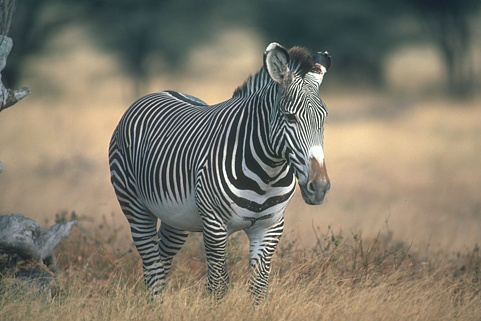
\includegraphics[width=\textwidth]{130066}
    \end{subfigure}
    ~ %add desired spacing between images, e. g. ~, \quad, \qquad, \hfill etc. 
      %(or a blank line to force the subfigure onto a new line)
    \begin{subfigure}[b]{0.2\textwidth}
        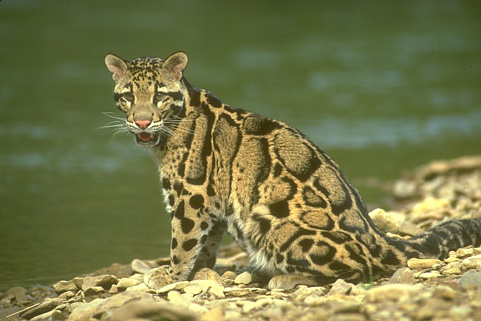
\includegraphics[width=\textwidth]{160067}
    \end{subfigure} \\[2ex]       
    
    \begin{subfigure}[t]{\dimexpr0.2\textwidth+20pt\relax}
    	\makebox[20pt]{\raisebox{25pt}{ \rotatebox[origin=c]{90} {\small \textsf{\textbf{150 sp}}} }}%
    	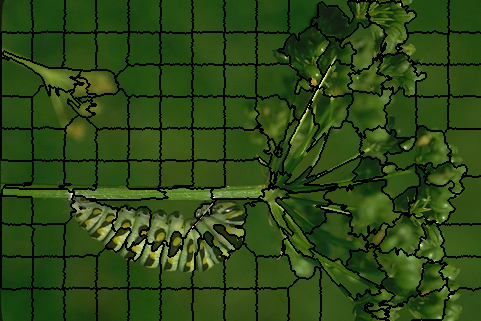
\includegraphics[width=\dimexpr\linewidth-20pt\relax]{35028_wt_150_segs} 
    \end{subfigure}      
    ~ %add desired spacing between images, e. g. ~, \quad, \qquad, \hfill etc. 
      %(or a blank line to force the subfigure onto a new line)
    \begin{subfigure}[b]{0.2\textwidth}
        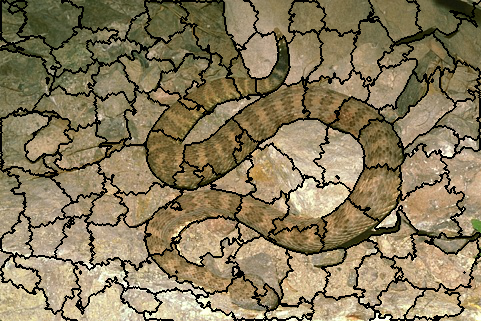
\includegraphics[width=\textwidth]{87015_wt_150_segs}
    \end{subfigure}
    ~ %add desired spacing between images, e. g. ~, \quad, \qquad, \hfill etc. 
      %(or a blank line to force the subfigure onto a new line)
    \begin{subfigure}[b]{0.2\textwidth}
        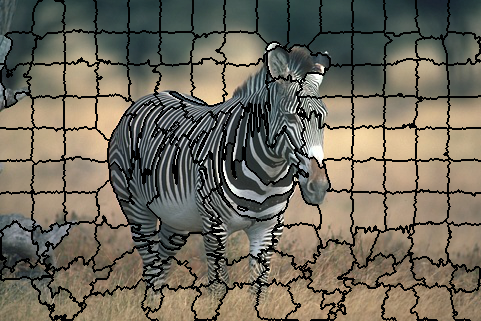
\includegraphics[width=\textwidth]{130066_wt_150_segs}
    \end{subfigure}
    ~ %add desired spacing between images, e. g. ~, \quad, \qquad, \hfill etc. 
      %(or a blank line to force the subfigure onto a new line)
    \begin{subfigure}[b]{0.2\textwidth}
        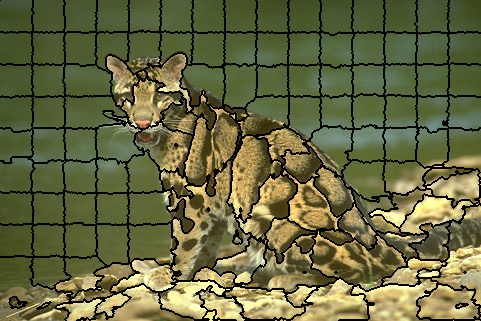
\includegraphics[width=\textwidth]{160067_wt_150_segs}
    \end{subfigure} \\ [2ex]
    
    \begin{subfigure}[t]{\dimexpr0.2\textwidth+20pt\relax}
    	\makebox[20pt]{\raisebox{25pt}{ \rotatebox[origin=c]{90} {\small \textsf{\textbf{300 sp}}} }}%
    	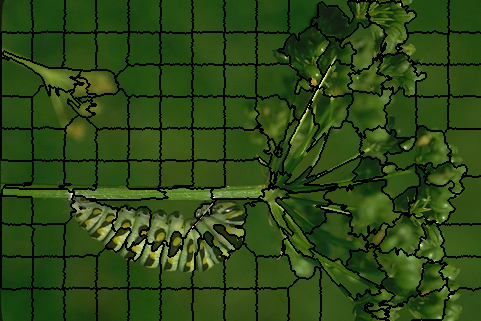
\includegraphics[width=\dimexpr\linewidth-20pt\relax]{35028_wt_150_segs} 
    \end{subfigure}      
    ~ %add desired spacing between images, e. g. ~, \quad, \qquad, \hfill etc. 
      %(or a blank line to force the subfigure onto a new line)
    \begin{subfigure}[b]{0.2\textwidth}
        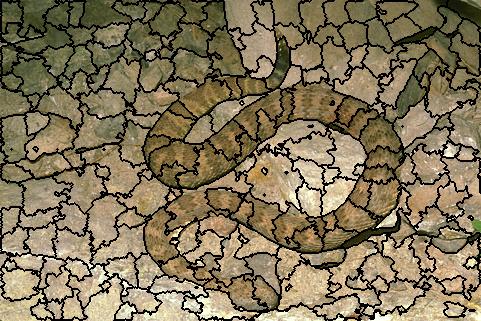
\includegraphics[width=\textwidth]{87015_wt_300_segs}
    \end{subfigure}
    ~ %add desired spacing between images, e. g. ~, \quad, \qquad, \hfill etc. 
      %(or a blank line to force the subfigure onto a new line)
    \begin{subfigure}[b]{0.2\textwidth}
        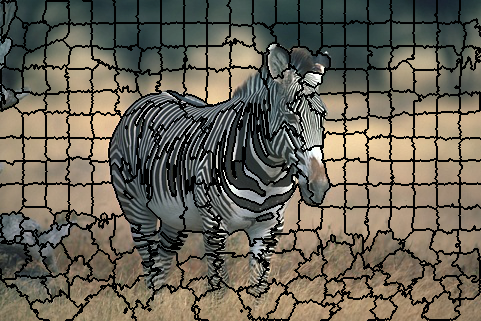
\includegraphics[width=\textwidth]{130066_wt_300_segs}
    \end{subfigure}
    ~ %add desired spacing between images, e. g. ~, \quad, \qquad, \hfill etc. 
      %(or a blank line to force the subfigure onto a new line)
    \begin{subfigure}[b]{0.2\textwidth}
        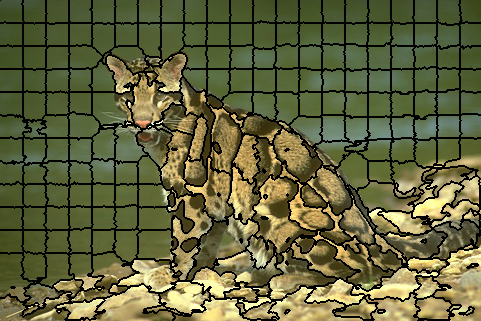
\includegraphics[width=\textwidth]{160067_wt_300_segs}
    \end{subfigure} \\ [2ex]
    
    \begin{subfigure}[t]{\dimexpr0.2\textwidth+20pt\relax}
    	\makebox[20pt]{\raisebox{25pt}{ \rotatebox[origin=c]{90} {\small \textsf{\textbf{600 sp}}} }}%
    	\includegraphics[width=\dimexpr\linewidth-20pt\relax]{35028_wt_600_segs} 
    \end{subfigure}      
    ~ %add desired spacing between images, e. g. ~, \quad, \qquad, \hfill etc. 
      %(or a blank line to force the subfigure onto a new line)
    \begin{subfigure}[b]{0.2\textwidth}
        \includegraphics[width=\textwidth]{87015_wt_600_segs}
    \end{subfigure}
    ~ %add desired spacing between images, e. g. ~, \quad, \qquad, \hfill etc. 
      %(or a blank line to force the subfigure onto a new line)
    \begin{subfigure}[b]{0.2\textwidth}
        \includegraphics[width=\textwidth]{130066_wt_600_segs}
    \end{subfigure}
    ~ %add desired spacing between images, e. g. ~, \quad, \qquad, \hfill etc. 
      %(or a blank line to force the subfigure onto a new line)
    \begin{subfigure}[b]{0.2\textwidth}
        \includegraphics[width=\textwidth]{160067_wt_600_segs}
    \end{subfigure}     

	\caption{}\label{fig:wt_suprepixels}    
\end{figure}


\subsubsection{SLIC superpixels}
The Simple Linear Iterative Clustering (SLIC) algorithm is part of the superpixel clustering-based methods. The methods in this category group pixels into clusters (superpixels) and iteratively refine such clusters until some convergence criterion is met. In the case of the SLIC, the centers of the clusters are randomly initialized and then associate each pixel to the closest central pixel. The central clusters are subsequently adjusted iteratively until the error converges.

The SLIC algorithm allows to control the number of superpixels (approximately) to be found in the image; the compactness of the superpixels and the as well as the adherence to the boundaries of the objects. However, this method cannot capture the global properties of the image \citep{Stutz.Hermans.ea:CVIU:2018}. Figure \ref{fig:slic_suprepixels} shows, in the same way as the previous algorithms, the results of the method asking for 150, 300 and 600 superpixels.


\begin{figure}[!ht]
    \centering
    \begin{subfigure}[t]{\dimexpr0.2\textwidth+20pt\relax}
    	\makebox[20pt]{\raisebox{25pt}{ \rotatebox[origin=c]{90} {\small \textsf{\textbf{Input image}}} }}%
    	\includegraphics[width=\dimexpr\linewidth-20pt\relax]{35028} 
    \end{subfigure}      
    ~ %add desired spacing between images, e. g. ~, \quad, \qquad, \hfill etc. 
      %(or a blank line to force the subfigure onto a new line)
    \begin{subfigure}[b]{0.2\textwidth}
        \includegraphics[width=\textwidth]{87015}
    \end{subfigure}
    ~ %add desired spacing between images, e. g. ~, \quad, \qquad, \hfill etc. 
      %(or a blank line to force the subfigure onto a new line)
    \begin{subfigure}[b]{0.2\textwidth}
        \includegraphics[width=\textwidth]{130066}
    \end{subfigure}
    ~ %add desired spacing between images, e. g. ~, \quad, \qquad, \hfill etc. 
      %(or a blank line to force the subfigure onto a new line)
    \begin{subfigure}[b]{0.2\textwidth}
        \includegraphics[width=\textwidth]{160067}
    \end{subfigure} \\[2ex]       
    
    \begin{subfigure}[t]{\dimexpr0.2\textwidth+20pt\relax}
    	\makebox[20pt]{\raisebox{25pt}{ \rotatebox[origin=c]{90} {\small \textsf{\textbf{150 sp}}} }}%
    	\includegraphics[width=\dimexpr\linewidth-20pt\relax]{35028_slic_150_segs} 
    \end{subfigure}      
    ~ %add desired spacing between images, e. g. ~, \quad, \qquad, \hfill etc. 
      %(or a blank line to force the subfigure onto a new line)
    \begin{subfigure}[b]{0.2\textwidth}
        \includegraphics[width=\textwidth]{87015_slic_150_segs}
    \end{subfigure}
    ~ %add desired spacing between images, e. g. ~, \quad, \qquad, \hfill etc. 
      %(or a blank line to force the subfigure onto a new line)
    \begin{subfigure}[b]{0.2\textwidth}
        \includegraphics[width=\textwidth]{130066_slic_150_segs}
    \end{subfigure}
    ~ %add desired spacing between images, e. g. ~, \quad, \qquad, \hfill etc. 
      %(or a blank line to force the subfigure onto a new line)
    \begin{subfigure}[b]{0.2\textwidth}
        \includegraphics[width=\textwidth]{160067_slic_150_segs}
    \end{subfigure} \\ [2ex]
    
    \begin{subfigure}[t]{\dimexpr0.2\textwidth+20pt\relax}
    	\makebox[20pt]{\raisebox{25pt}{ \rotatebox[origin=c]{90} {\small \textsf{\textbf{300 sp}}} }}%
    	\includegraphics[width=\dimexpr\linewidth-20pt\relax]{35028_slic_150_segs} 
    \end{subfigure}      
    ~ %add desired spacing between images, e. g. ~, \quad, \qquad, \hfill etc. 
      %(or a blank line to force the subfigure onto a new line)
    \begin{subfigure}[b]{0.2\textwidth}
        \includegraphics[width=\textwidth]{87015_slic_300_segs}
    \end{subfigure}
    ~ %add desired spacing between images, e. g. ~, \quad, \qquad, \hfill etc. 
      %(or a blank line to force the subfigure onto a new line)
    \begin{subfigure}[b]{0.2\textwidth}
        \includegraphics[width=\textwidth]{130066_slic_300_segs}
    \end{subfigure}
    ~ %add desired spacing between images, e. g. ~, \quad, \qquad, \hfill etc. 
      %(or a blank line to force the subfigure onto a new line)
    \begin{subfigure}[b]{0.2\textwidth}
        \includegraphics[width=\textwidth]{160067_slic_300_segs}
    \end{subfigure} \\ [2ex]
    
    \begin{subfigure}[t]{\dimexpr0.2\textwidth+20pt\relax}
    	\makebox[20pt]{\raisebox{25pt}{ \rotatebox[origin=c]{90} {\small \textsf{\textbf{600 sp}}} }}%
    	\includegraphics[width=\dimexpr\linewidth-20pt\relax]{35028_slic_600_segs} 
    \end{subfigure}      
    ~ %add desired spacing between images, e. g. ~, \quad, \qquad, \hfill etc. 
      %(or a blank line to force the subfigure onto a new line)
    \begin{subfigure}[b]{0.2\textwidth}
        \includegraphics[width=\textwidth]{87015_slic_600_segs}
    \end{subfigure}
    ~ %add desired spacing between images, e. g. ~, \quad, \qquad, \hfill etc. 
      %(or a blank line to force the subfigure onto a new line)
    \begin{subfigure}[b]{0.2\textwidth}
        \includegraphics[width=\textwidth]{130066_slic_600_segs}
    \end{subfigure}
    ~ %add desired spacing between images, e. g. ~, \quad, \qquad, \hfill etc. 
      %(or a blank line to force the subfigure onto a new line)
    \begin{subfigure}[b]{0.2\textwidth}
        \includegraphics[width=\textwidth]{160067_slic_600_segs}
    \end{subfigure}     

	\caption{}\label{fig:slic_suprepixels}    
\end{figure}


\section{Perceptual image boundaries}


\subsection{Earth Mover's Distance for non-normalized distributions}
We have seen the utility of EMD in Chapter \ref{ch:similarity_measures} as a true metric for measuring similarity between distributions. In image search systems based on color information, EMD is capable of measuring small changes in the normalized color distributions of superhero images. On the other hand, with the texture imagettes, the EMD is able to capture, reflect and measure the importance of the logarithmic (frequency) and polar (orientation) axes of the texture signature (see figure \ref{fig:MDS_EMD}  in appendix \ref{ch:suplementary_material_retrieval_systems}). 


\subsubsection{Ground distance matrix}


\begin{figure}[!ht]
    \centering
    \begin{subfigure}[b]{0.47\textwidth}
		\includegraphics[width=\textwidth]{ground_distance_matrix_euclidean}	
		\caption{Euclidean}
        \label{fig:ground_distance_matrix_euclidean}
	\end{subfigure}
	~ %add desired spacing between images, e. g. ~, \quad, \qquad, \hfill etc. 
    %(or a blank line to force the subfigure onto a new line)
    \begin{subfigure}[b]{0.47\textwidth}
		\includegraphics[width=\textwidth]{ground_distance_matrix_sqeuclidean}	
		\caption{Squared euclidean}
        \label{fig:ground_distance_matrix_sqeuclidean}
	\end{subfigure} \\[2ex]
    
    \begin{subfigure}[b]{0.47\textwidth}
		\includegraphics[width=\textwidth]{ground_distance_matrix_lin_polar}	
		\caption{Linear-polar}
        \label{fig:ground_distance_matrix_lin_polarc}
	\end{subfigure}  
	~ %add desired spacing between images, e. g. ~, \quad, \qquad, \hfill etc. 
    %(or a blnk line to force the subfigure onto a new line)
	\begin{subfigure}[b]{0.47\textwidth}
		\includegraphics[width=\textwidth]{ground_distance_matrix_log_polar}	
		\caption{Log-polar}
        \label{fig:ground_distance_matrix_log_polar}
	\end{subfigure}  
	   
   \caption{Visualizations of cost matrix of EMD.}
   \label{fig:EMD_ground_distance_matrix}
\end{figure}

\subsection{Image segmentation based on image gradients}
\subsubsection{MST threshold graph-cut}
This method is based on the graph cut using a threshold value. However, the choice of this threshold value is not always obvious, and this value may differ for each image.
We propose obtaining a threshold value by fitting a probability density function to the values of the egdes of the image graph. Our hypothesis is that the areas with the same color and / or texture information behave as flat areas in the generated feature space, therefore those edges that connect these areas behave as outliers within the probability function. Under this principle, we can propose a cut at some quantile level of the distribution, for example, to 90\%.

In addition, to increase the visibility of outliers, we reduce the number of edges by applying the distribution of the function on the minimun spaning tree (MST) of the k-nn graph.

%\begin{figure}[!ht]
%\centering
%\includegraphics[width=0.4\textwidth]{cow_mst_weight_dist.png} \caption{Weight distribution of the edges of the MST of an image.  On the values we fit a log-norm probability function}
%\end{figure}\label{fig:gradient_computation_diagram}
%
%\begin{tabular}{ccc}
%\includegraphics[width=0.33\textwidth]{8068_graphcut_result.png}  & \includegraphics[width=0.33\textwidth]{15062_graphcut_result.png} & \includegraphics[width=0.33\textwidth]{48017_graphcut_result.png}\\
%\end{tabular}


\subsubsection{Spectral clustering}
To apply this segmentation method, we obtain a affinity matrix from the adjacency matrix generated from the connections of the k-nn graph. The normalization of the affinity matrix is a prerequisite for achieving image segmentation. To achieve this, we apply a global normalization with a sigma parameter.

%\begin{tabular}{ccc}
%\includegraphics[width=0.33\textwidth]{8068_spec_result.png}  & \includegraphics[width=0.33\textwidth]{15062_spec_result.png} & \includegraphics[width=0.33\textwidth]{48017_spec_result.png}\\
%\end{tabular}

\subsubsection{Normalized graph-cut}
In the same way as the spectral clustering method, the normalized slicing method uses a normalized affinity matrix. The differences between these two methods lie in the speed of calculation and the need to define a number of clusters. In the case of spectral clustering, the calculation time is less, however, it is necessary to give an estimated number of regions to find.

\subsubsection{Gradient-based segmentation comparison}

Taking into account the great variety of techniques, models, strategies and their respective parameters used in this work, we wanted to cover the widest possible range of variables in our tests.

Therefore, to evaluate the learning of the importance of color and texture and to have a qualitative score, we calculated the F-score using the segmentation results of each method mentioned above. The calculation of such a score can be done individually, that is, by image, however, we collect the set of scores from the BSD test subset and use them in some box plots. These graphs first show the precision and recall of each method, but it also allows us to see which Gabor space configuration gives the best results.


%\includegraphics[width=\textwidth]{Thr_graphcut_Fscores_log_mst_boxplot_pred_linreg.png}  \\
%Scores using the gradients predicted by the linear regression model (LinReg) and the Threshold graph cut method\\
%\includegraphics[width=\textwidth]{Thr_graphcut_Fscores_log_mst_boxplot.png} \\
%Scores using the sum of the computed gradients and the Threshold graph cut method\\
%\includegraphics[width=\textwidth]{Spectral_clustering_Fscores_global_complete_boxplot_pred_linreg.png} \\
%Scores using the gradients predicted by the linear regression model (LinReg) and the Spectral Clustering method\\
%\includegraphics[width=\textwidth]{Spectral_clustering_Fscores_global_complete_boxplot.png}\\
%Scores using the sum of the computed gradients and the Spectral Clustering method\\

\section{Perceptual image segmentation}
\subsection{Hierarchical watershed}
\subsection{Interactive image segmentation}



\section{Comparison with the state of the art}
\subsection{Scores}

\subsubsection{Precision-Recall curve and Average Precision (AP)}
\subsubsection{Optimal Dataset Scale (ODS), Optimal Image Scale (OIS)}
\subsubsection{Probabilistic Rand Index (PRI)}
\subsubsection{Variation of Information(VI)}

\subsubsection{}

\begin{table}[]
\centering
\begin{tabular}{c|c|c|c||c|c|c|}
\cline{2-7}
                                  & \multicolumn{3}{c||}{\textbf{BSDS300}} & \multicolumn{3}{c|}{\textbf{BSDS500}} \\ \cline{2-7} 
                                  & ODS         & OIS        & AP         & ODS         & OIS        & AP         \\ \hline
\multicolumn{1}{|c|}{Human}       & 0.79        & 0.79       & -          & 0.80        & 0.80       & -          \\ \hline
\multicolumn{1}{|c|}{Ours}        & 0.65        & 0.67       & 0.62       & 0.66        & 0.68       & 0.62       \\
\multicolumn{1}{|c|}{Mean Shift}  & 0.63        & 0.66       & 0.54       & 0.64        & 0.68       & 0.56       \\
\multicolumn{1}{|c|}{Felz-Hutt}   & 0.58        & 0.62       & 0.53       & 0.61        & 0.64       & 0.56       \\
\multicolumn{1}{|c|}{NCuts}       & 0.62        & 0.66       & 0.43       & 0.64        & 0.68       & 0.45       \\
\multicolumn{1}{|c|}{Canny}       & 0.58        & 0.62       & 0.58       & 0.60        & 0.63       & 0.58       \\
\multicolumn{1}{|c|}{Pb}          & 0.65        & -          & -          & -           & -          & -          \\ \hline
\multicolumn{1}{|c|}{mPb}         & 0.67        & -          & -          & -           & -          & -          \\
\multicolumn{1}{|c|}{sPb}         & 0.68        & -          & -          & -           & -          & -          \\
\multicolumn{1}{|c|}{gPb}         & 0.70        & 0.72       & 0.66       & 0.71        & 0.74       & 0.65       \\
\multicolumn{1}{|c|}{gPb-owt-ucm} & 0.73        & 0.76       & 0.73       & 0.73        & 0.76       & 0.73       \\ \hline
\end{tabular}
\end{table}


\begin{table}[]
\centering
\begin{tabular}{c|c|c|c||c|c||c|c|}
\cline{2-8}
                                  & \multicolumn{7}{c|}{\textbf{BSDS500}}                                                                                       \\ \cline{2-8} 
                                  & \multicolumn{3}{c||}{Covering $(\uparrow)$} & \multicolumn{2}{c||}{PRI $(\uparrow)$} & \multicolumn{2}{c|}{VI $(\downarrow)$} \\ \cline{2-8} 
                                  & ODS          & OIS          & Best         & ODS               & OIS               & ODS                & OIS               \\ \hline
\multicolumn{1}{|c|}{Human}       & 0.72         & 0.72         & -            & 0.88              & 0.88              & 1.17               & 1.17              \\ \hline
\multicolumn{1}{|c|}{Ours}        & 0.56         & 0.60         & 0.67         & 0.81              & 0.83              & 1.79               & 1.57              \\ \hline
\multicolumn{1}{|c|}{gPb-owt-ucm} & 0.59         & 0.65         & 0.74         & 0.83              & 0.86              & 1.69               & 1.48              \\ \hline
\multicolumn{1}{|c|}{Mean Shift}  & 0.54         & 0.58         & 0.66         & 0.79              & 0.81              & 1.85               & 1.64              \\ \hline
\multicolumn{1}{|c|}{Felz-Hutt}   & 0.52         & 0.57         & 0.69         & 0.80              & 0.82              & 2.21               & 1.87              \\ \hline
\multicolumn{1}{|c|}{Ncuts}       & 0.45         & 0.53         & 0.67         & 0.78              & 0.80              & 2.23               & 1.89              \\ \hline
\end{tabular}
\end{table}

\begin{figure}[!ht]
	\centering
	\includegraphics[width=\textwidth]{pr_curves_mymethod}
	\caption{Precision-recall plot of different contour detectors.}\label{fig:pr_curves}
\end{figure}
\subsection{Results}


\section{Importance of color and texture in image segmentation}


\section{Conclusions}
